% This is "aamas2014.tex", a revised version of aamas2013.tex
% This file should be compiled with "aamas2014.cls"
% This example file demonstrates the use of the 'aamas2014.cls'
% LaTeX2e document class file. It is for those submitting
%File: formatting-instruction.tex
\documentclass[letterpaper]{article}
\usepackage{aaai}
%\usepackage{times}
\usepackage[ruled, vlined, linesnumbered]{algorithm2e}
\DontPrintSemicolon

\usepackage{graphics,amsmath,amssymb}
\usepackage{times}
\usepackage{url}

\nocopyright
 \def\baselinestretch{0.95}
\setlength{\pdfpagewidth}{8.5in}
\setlength{\pdfpageheight}{11in}
\pdfinfo{
/Title Human-Agent Collaboration for Real-World Disaster Response
/Author Tracking No. XXX}
\setcounter{secnumdepth}{0}
\frenchspacing
 \begin{document}
\setlength{\abovecaptionskip}{2pt}
\setlength{\belowcaptionskip}{-6pt}
\setlength{\abovedisplayskip}{0pt}
\setlength{\belowdisplayskip}{0pt}
\setlength{\floatsep}{0pt}
\setlength{\textfloatsep}{10pt}
% The file aaai.sty is the style file for AAAI Press
% proceedings, working notes, and technical reports.
%

\title{Human-Agent Collaboration for Real-World Disaster Response}
\author{Tracking No. XXX}

 \maketitle

\begin{abstract}
In this paper, we develop an algorithm to solve the problem of  coordinating emergency responders in uncertain environments and evaluate it in a novel mixed-reality game called AtomicOrchid. Specifically, the algorithm is used by a software  agent that works alongside a human commander to guide human players to complete rescue tasks. More importantly, we study the interactions between the human players and the agent in real-time and show that it improves  performance significantly (compared to a no-agent setting). Our results allow us to specify design guidelines for human-agent collaboration in such settings.
 \end{abstract}\vspace{-3mm}

% Note that the category section should be completed after reference to the ACM Computing Classification Scheme available at
% http://www.acm.org/about/class/1998/.

%\keywords{Human-Agent Interaction, Agents for improving human cooperative activities, Disaster Response.}
%\vspace{-2mm}
\section{Introduction}
The coordination of teams of field responders in search and rescue missions is regarded as one  of the grand challenges for multi-agent systems research \cite{kitano}. In such settings, responders with different capabilities (e.g., fire extinguishing, digging, or life support) have to form teams in order to perform rescue tasks (e.g., extinguishing a fire or digging civilians out of rubble or both) to minimise  costs (e.g., time or money) and maximise the number of lives and buildings saved. Thus, responders have to plan their paths to the tasks (as these may be distributed in space) and form specific teams  to complete some tasks. These teams, in turn, may  need to disband and reform other teams to complete other tasks requiring different capabilities, taking into account the status (e.g., health or building fire) of the tasks and the environment (e.g., if a fire or radioactive cloud is spreading). Furthermore, uncertainty in the environment (e.g., wind direction or speed) or in the responders' abilities to complete tasks (e.g., some may be tired or get hurt) means that plans may need to change depending on the state of the players and the environment. 

To address these challenges, in recent years, a number of algorithms and mechanisms have been developed to create teams and allocate tasks. For example, \cite{ramchurn:teal:2010,koes:teal:2005,scerri:teal:200X} and \cite{ramchurn:robocup:2010,chapman:teal:2010}, developed centralised and decentralised optimisation algorithms respectively to allocate rescue tasks efficiently to teams of field responders with different capabilities. However, none of these approaches considered the uncertainty in the environment or in the field responders' abilities. Crucially, to date, while all of these algorithms have been shown to perform well in simulations (assuming agents as computational entities), none of them have been \emph{deployed} to guide \emph{real} human responders (amateur or expert) in real-time rescue missions. Thus, it is still unclear whether these algorithms will cope with real-world uncertainties (e.g., communication breakdowns or change in wind direction), be acceptable to humans (i.e., agent-computed plans are not confusing and take into account human capabilities), and do help humans perform better than on their own.

Against this background, in this paper we develop a novel algorithm for team coordination under uncertainty and evaluate it within a real-world mixed-reality game that embodies the simulation of team coordination in disaster response settings. In more detail, we consider scenario involving rescue tasks distributed in a disaster space over which a radioactive cloud is spreading. Tasks need to be completed by the responders before the area is completely covered by the cloud (as responders will die from radiation exposure) which is spreading according to varying wind speed and direction. Our algorithm captures the uncertainty in the scenario (i.e., in terms of environment and player states) and  is able to compute a policy to allocate responders to tasks to minimise the time to complete all tasks without them being exposed to significant radiation. The algorithm is then used by an agent to guide human responders based on their perceived states. This agent is then implemented in our deployed platform, AtomicOrchid, that structures the interaction between human responders, a human coordinator, and the agent in a mixed-reality location-based game. By so doing, we are able to study, both quantitatively and qualitatively, the performance of a mixed-initiative team (i.e., a human team under human and agent guidance)  and the interactions between the different actors in the system. Thus, this paper advances the state of the art in the following ways:
\begin{enumerate}
\item We develop a novel approximate algorithm for team formation under uncertainty using a Multi-agent Markov Decision Process (MMDP) paradigm, and show how it accounts for real-world uncertainties.
\item We present AtomicOrchid, a novel platform to evaluate team formation under uncertainty using the concept of mixed-reality games. AtomicOrchid allows an agent, using our team formation algorithm, to coordinate, in real-time, human players using mobile phone-based messaging, to complete rescue tasks efficiently.
\item We provide the first real-world evaluation of a team formation agent in a disaster response setting in field trials and present both quantitative and qualitative results. Our results allow us to elucidate some of the challenges for the formation of human-agent collectives, that is, mixed-initiative teams where control can be passed between agents and humans in flexible ways.
\end{enumerate}
When taken together, our results show, for the first time, how agent-based coordination algorithms for disaster response can be validated in the real-world. Moreover, these results allow us to derive a methodology and guidelines to evaluate human-agent interaction in real-world settings. 

The rest of this paper is structured as follows. Section \ref{sec:scenario} formalises the disaster response problem as an MMDP. Section \ref{sec:algorithm} then describes the algorithm to solve the path planning and task allocation problems presented by the MMDP while Section \ref{sec:atomic} describes the AtomicOrchid platform. Section \ref{sec:evaluation} presents our pilot study and the evaluation of the system in a number of field trials.  Finally, Section \ref{sec:conclusions} concludes.
\section{The Disaster Scenario}

\noindent We consider a disaster scenario involving a satellite, containing radioactive fuel, that has crashed in a sub-urban area (see Section \ref{atomic} to see how this helps implement a credible mixed-reality game). While debris is strewn around a large area, damaging buildings and causing accidents and injuring civilians, radioactive discharge from the debris is gradually spreading over the area, threatening to contaminate food reserves and people. Hence, emergency services, voluntary organisations, and the military are deployed to help evacuate the casualties and resources before these are engulfed by  radioactive cloud.  In what follows, we model this scenario formally and then describe the optimisation problem faced by the actors (i.e., including emergency services, volunteers, medics, and soldiers) in trying to save as many lives and resources as they can.

\subsection{Formal Model}
\noindent Let $G$ denote a grid overlaid on top of the disaster space, and the satellite and actors are located at various coordinates $(x,y) \in G$ in this grid. The set of field responders be denoted as $i_1, \cdots, i_n \in I$ and the set of rescue tasks as  $t_1,\cdots, t_m\in T$.  As responders enact tasks, they may become tired or get injured. Hence, we assign each responder  a health level $h_i\in [0,100]$. Moreover, each responder will have  a specific role  $r \in Roles$ (e.g., fire brigade, soldier, or medic) and this will determine the capabilities he or she has and therefore the tasks he or she can perform. We denote as $Roles(i)$ the role of responder $i$. In turn, to complete a given task $t$,  a set of responders $I' \subseteq I$ with specific roles $R_t \subseteq R$ is required. Thus, a task can only be completed by a team of responders $I'$ if $\{Roles(i) | i \in I'\} = R_t$. 

Given this model, we next formulate the optimisation problem faced by the responders (and later solved in Section \ref{sec:algo}). To this end, we propose a Multi-Agent Markov Decision Process (MMDP)~\cite{?} that captures the uncertainties of the radiative cloud and the responders' behaviours. Specifically, we model the spreading of the radiative cloud as a random process over the spatial space and allow the responders' actions to be failed or delayed during the rescue process. Other existing models for rescue tasks such as CFSTP~\cite{?} and HTSSC~\cite{?} cannot be applied to our problem as they usually require the process of task executions to be deterministic. They need to explicitly model the time limit of a task and the duration of completing a task by the responders as spatial and temporal constraints, which are stochastic in our domain. Instead, in the MMDP model, we represent the task executions as stochastic processes of state transitions. Thus, the uncertainties of the radiative cloud and the responders' behaviours can be straightforwardly captured with transition probabilities. Additionally, modeling the problem as a MMDP enables us to use many sophisticated algorithms that have already been developed in the literature.

\subsection{Radiation Cloud Modelling}\label{sec:radiation}
\noindent The radiation cloud is assumed to be monitored using a number of sensors on the ground (within the disaster space) that collect readings of the radiation cloud intensity and wind velocity every minute of the game. These sensors can be at fixed locations or held by mobile agents.  The radiation cloud diffusion process is modelled in a standard way by a nonlinear Markov field stochastic differential equation,  
\begin{eqnarray*}
\frac{D \text{Rad}({\bf z}, \tau)}{D \tau}=\kappa \triangledown^2 \text{Rad}({\bf z},\tau)-\text{Rad}({\bf z},\tau)\triangledown \cdot {\bf w}({\bf z},\tau)+\sigma({\bf z},\tau)
\end{eqnarray*}
where $D$ is the material derivative, $\text{Rad}({\bf z},\tau)$ is the radiation cloud intensity at location ${\bf z}$ at time $\tau$, $\kappa$ is a fixed diffusion coefficient and $\sigma$ is the radiation source(s) emission rate. The diffusion equation is solved on a regular grid defined across the environment with grid coordinates $G$ (as defined in Section \ref{sec:model}).  Furthermore, the grid is solved at discrete time instances $\tau$.  The cloud is driven by wind forces which vary both spatially and temporally.  These forces induce anisotropy into the cloud diffusion process which is proportional to the wind velocity, ${\bf w}({\bf z},\tau)$.  The wind velocity is drawn from two independent Gaussian processes (GP), one GP for each Cartesian coordinate axis, $w_i({\bf z},\tau)$, of ${\bf w}({\bf z},\tau)$.  The GP captures both the spatial distribution of the wind velocity and the dynamic process resulting from shifting wind patterns such as short term gusts and longer term variations. 

% In our simulation, each spatial wind velocity component is modelled by a squared-exponential GP covariance function, $K$, with fixed input and output scales (although any covariance function can be substituted). Furthermore, as wind conditions may change over time we introduce a temporal correlation coefficient, $\rho$, to the covariance function.  Thus, for a single component, $w_i$, of ${\bf w}$, defined over grid $G$ at times $\tau$ and $\tau^\prime$, the wind process covariance function is, $\text{Cov}(w_i(G,\tau),w_i(G,\tau^\prime))=\rho(\tau,\tau^\prime) K(G,G)$.  We note that, when $\rho=1$ the wind velocities are time invariant (although spatially variant).  Values of $\rho<1$ model wind conditions that change over time.

Using the above model, we are able to create a moving radiation cloud, thus posing a real challenge both for the HQ (agent and commander) and the responders on the ground, as predictions they can make of where the cloud will move to will be prone to uncertainty both to the simulated wind speed and direction. 


%(\textbf{Steve: in the platform we take the `real' values from the diffusion process i believe. Does the above capture this? We will say that we will add the features you mention below to a future version of the platform where we aim to do both situational awareness and rescue. Add a sentence above to conclude where we took the values from and the process takes into account the  location of radiation source. Also, your notation clashes with the notations in the scenario and Feng's algorithm - please try to align.}
%The cloud intensity and wind velocity are measured by {\it monitor agents} equipped with geiger-counters and anemometers.  These agents are directed to take measurements with greatest information gain in the radiation cloud intensity.  The measurements are folded into the EKF and this refines estimates of the radiation cloud across the grid.  Figure~\ref{radiation_screen_shots} shows example cloud simulations for slow varying (i.e. $\rho=0.99$) and gusty (i.e. $\rho=0.90$) wind conditions.  Figure~\ref{radiation_screen_shots}(a) shows slow varying wind conditions in which case the radiation cloud can be interpolated accurately using sparse sensor measurements and the LFM model.  Alternatively, during gusty conditions the radiation cloud model is more uncertain far from the locations where recent measurements have been taken, as shown in Figure~\ref{radiation_screen_shots}(b).
%
%\begin{figure}[ht] \begin{center}
%    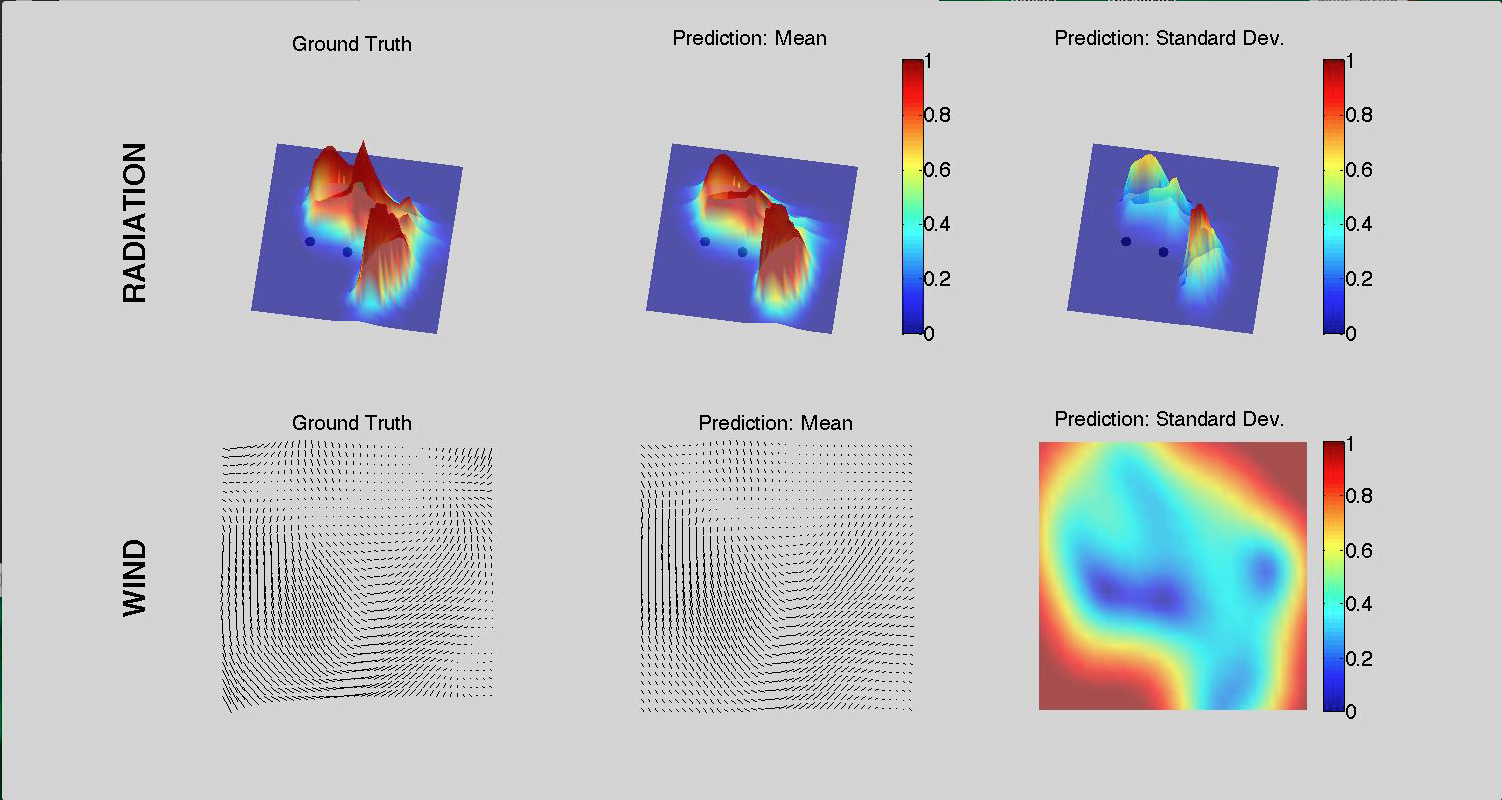
\includegraphics[width=0.45\textwidth]{figures/radiation_ss_calm.png}\\
%    (a) Slowly varying wind conditions\\ \ \\
%    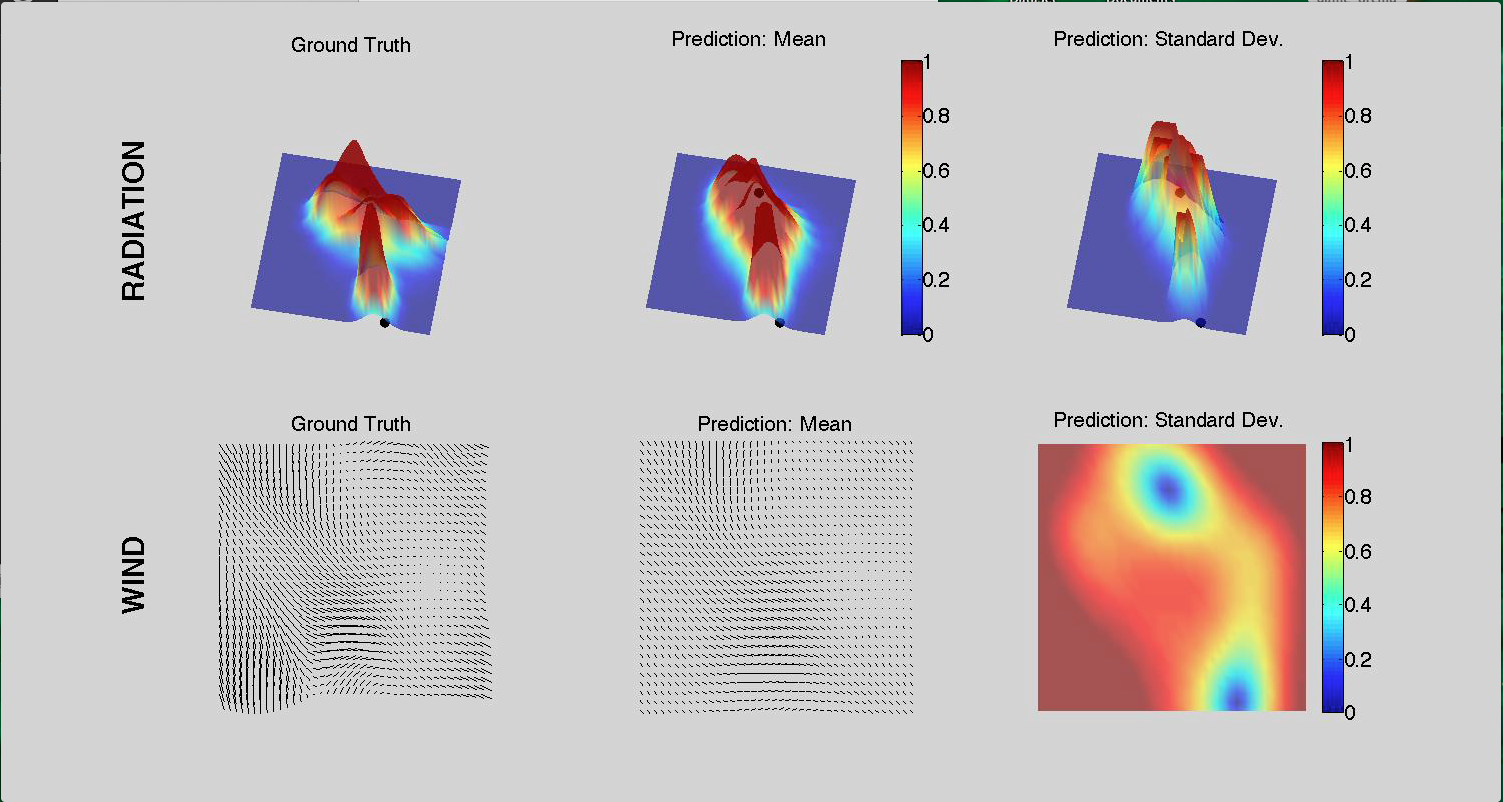
\includegraphics[width=0.45\textwidth]{figures/radiation_ss_gust.png}\\
%    (b) Gusty wind conditions 
%\caption{\label{radiation_screen_shots} Radiation and wind simulation ground truth and EKF estimates obtained using measurements from monitor agents (black dots).  Left most panes are ground truth radiation and wind conditions, the middle panes are corresponding estimates and right most panes are state uncertainties:  (a) Invariant and (b) gusty wind conditions.}
%\end{center}
%\end{figure}

\subsection{The Optimisation Problem}
\label{sec:model}
\noindent Previous agent-based models for team coordination in disaster response typically assume deterministic task executions and environments \cite{ramchurn:etal:2010,Scerri2005}. However, in order to evaluate agent-guided coordination in a real-world environment, it is important to consider uncertainties due to player behaviours and the environment (as discussed in the previous section). Given this, we propose a new representation for the task allocation problem in disaster response that does take into account such uncertainties. More specifically, we represent this problem using an MMDP that captures the uncertainties of the radioactive cloud and the responders' behaviours. We model the spreading of the radioactive cloud as a random process over the disaster space and allow the actions requested from the responders to  fail (because they decline to go to a  task) or incur delays (because they are too slow) during the rescue process. Thus in the MMDP model, we represent  task executions as stochastic processes of state transitions, while the uncertainties of the radioactive cloud and the responders' behaviours can be easily captured with transition probabilities.  More formally, the MMDP is
represented by tuple $\mathcal{M} = \langle I, S, \{A_i\}, P, R
\rangle$, where $I$ is the set of actors as defined in the previous
section,  $S$ is the state space, $A_i$ is a set of responder
$p_i$'s actions, $P$ is the transition function, and $R$ is the
reward function. We elaborate on each of these below.

In more detail, $S= S^G_r \times S_{p_1} \times \cdots \times
S_{p_n} \times S_{t_1} \times \cdots \times S_{t_m}$ where $S^G_r =
\{l_{(x,y)}| (x, y) \in G\}$ is the state variable of the
radioactive cloud that specifies the radioactive level
$l_{(x,y)}\in[0, 100]$ at every point $(x, y)\in G$. $S_{p_i} =
\langle h_i, (x_i, y_i), t_j \rangle$ is the state variable for
each responder $p_i$ that specifies her health level
$h_i\in[0, 100]$, her present position $(x_i, y_i)$, and the task
$t_j$ she is carrying out. $S_{t_j} = \langle {\tt st_j}, (x_j, y_j)
\rangle$ is then the state variable for task $t_j$ to specify its
status ${\tt st_j}$ (i.e., the target is picked up, dropped off, or idle) and position $(x_j, y_j)$. 

The three types of actions  (in set $A_i$) a responder can take
are: (i) {\em stay} in the current location $(x_i, y_i)$, (ii) {\em
move} to the 8 neighbouring locations, or (iii) {\em complete} a
task located at $(x_i, y_i)$. A joint action $\vec{a}=\langle a_1,
\cdots, a_n \rangle$ is a set of actions where $a_i\in A_i$, one
for each responder (a responder may just \emph{stay} at its current
position if it has no targets to rescue). The transition function
$P$ is defined in more detail as: $P= P_r \times P_{p_1} \times
\cdots \times P_{p_n} \times P_{t_1} \times \cdots \times P_{t_m}$
where:
\begin{itemize}
    \itemsep=-2pt
    \item $P_r(s'_r|s_r)$ is the probability the radioactive
        cloud spreads from state $s_r\in S^G_r$ to $s'_r\in
        S^G_r$. It captures the uncertainty of the  radiation
        levels in the environment due to  noisy sensor readings
        and the variations in wind speed and direction.
    \item $P_{p_i}(s'_{p_i}|s, a_i)$ is the probability
        responder $p_i$ transitions to a new state $s'_{p_i}\in
        S_{p_i}$ when executing action $a_i$. For example, when
        a responder is asked to go to a new location,  she
        may not end up there because  she is tired,
        gets injured, or receives radiation doses that are life
        threatening.
    \item $P_{t_j}(s'_{t_j}|s, \vec{a})$ is the probability
        of task $t_j$ being completed. A task $t_j$ can only be completed by a
        team of responders with the required types ($\Theta_{t_j}$) located at the
        same position as $t_j$.
\end{itemize}

Now,  if  $t_j$ is completed (i.e., in ${\tt st_j}\in S_{t_j}$, the
status ${\tt st_j}$ is marked as ``dropped off'' and its position $(x_j,
y_j)$ is within a safe zone), the team will be rewarded using
function $R$. The team is penalised if a responder $p_i$ gets
injured or receives a high dose of radiation (i.e., in $s_{p_i}$,
the health level $h_i$ is 0). Moreover, we attribute a cost to each
of the responders' actions since  each  action requires them to
exert some effort (e.g., running or carrying objects).


Give the above definitions, a policy for the MMDP is a mapping from
states to joint actions, $\pi: S \rightarrow \vec{A}$ so that the
responders know which actions to take given the current state of
the problem. The quality of a policy $\pi$ is  measured by
its expected value $V^\pi$, which can be computed recursively by
the Bellman equation:
\begin{equation}
  V^\pi(s^\tau) = R(s^\tau, \pi(s^\tau)) + \!\!\!\sum_{s^{\tau+1}\in S}\!\!\!
  P(s^{\tau+1}|s^\tau, \pi(s^t)) V^\pi(s^{\tau+1})
\end{equation}
where $\tau$ denotes the current time point and $\pi(s^\tau)$ is a joint action given $s^\tau$. The goal of solving
the MMDP is to find an optimal policy $\pi^*$ that maximises the
expected value with the initial state $s^0$, $\pi^* =
\arg\max_{\pi} V^\pi(s^0)$.

At each decision step, we assume the planning agent can fully
observe the state of the environment $s$ by collecting sensor
readings of the radioactive cloud and GPS locations of the
responders. Given a policy $\pi$ of the MMDP, a joint action
$\vec{a}=\pi(s)$ can be selected and broadcast to the responders
(as mentioned earlier).


\section{Team Coordination Algorithm}
\label{sec:algo}
Although the MMDP model captures the uncertainties of our
problem, it results in a very large search space making it
practically impossible to compute the optimal solution. Hence, we consider approximate solutions that result in
high quality allocations. To this end, we decompose $PA$'s
decision-making process into a hierarchical planning process: at the top level, a {\em task planning} algorithm is run
for the whole team to assign the best task to each responder given
the current state of the world; at the lower level, given a task, a
{\em path planning} algorithm is run by each responder to find the
best path to the task from her current location. Furthermore,
since not all states of MMDPs are relevant to the problem, we
only need to consider the reachable states given the current state.
Hence, we compute the policy online, starting from the current state
of the problem. This reduces computation significantly
because the number of the reachable states is usually much smaller
than the overall state space. In what follows, we describe each
level of our {\em online hierarchical planning} algorithm.

\subsection{Task Planning} \label{sec:taskplanning} As described earlier, each responder $p_i$ is of a specific type
$\theta_i \in \Theta$ that determines which task she can perform
and  a task $t$ can only be completed by a team of responders with
the required types $\Theta_t$. If, during the execution
of a plan, a responder $p_i$ is incapable of performing a task
(e.g., because she is tired or unclear where the task is), she
is removed from the set of responders under consideration
(that is $I \to I \setminus p_i$). This information can be obtained
from the state $s \in S$. When a task is completed by a chosen
team, the task is simply removed from the set (that is $T \to
T\setminus t_k$ if $t_k$ has been completed).

Now, to capture the efficiency of groupings of responders at
performing tasks, we define the value of a team $v(C_{jk})$ that
reflects the level of performance of team $C_k$ in performing task
$t_j$. This is computed from the estimated rewards that the team
obtains for performing $t_j$.  Then, the goal of the task planning
algorithm is to assign a task to each team that maximises the
overall team performance given the current state $s$, i.e.,
$\sum_{j=1}^m v(C_{j})$ where $C_j$ is a team for task $t_j$ and
$\{ C_1, \cdots, C_m \}$ is a {\em partition} of $I$ ($\forall
j\neq j', C_j \bigcap C_{j'} = \emptyset$ and $\bigcup_{j=1}^m
C_j=I$). In what follows, we first detail the procedure to compute
the value of all teams that are valid in a given state and then
detail the task allocation algorithm.


\subsubsection{Team Value Calculation}
The computation of  $v(C_{jk})$ for each team $C_{jk}$ is
challenging since there are many ways to configure teams and this needs to be done repeatedly (since there are more tasks than responders).
Moreover, a new policy must be computed after a given task $t_j$ is completed. This is time-consuming given the number of
states and joint actions. Hence, we propose to estimate
$v(C_{jk})$ through several simulations. This saves
computation as it avoids computing the complete policy to come
up with a good estimate of the team value, though we may not be
able to evaluate all possible future outcomes. According to the
central limit theorem, if the number of simulations is sufficiently
large, the estimated value will converge to the true $v(C_{jk})$.

Specifically, in each simulation, we first assign the responders in
$C_{jk}$ to task $t_j$ and run the simulator starting from the
current state $s$. After task $t_j$ is completed, the simulator
returns the sum of the rewards $r$ and the new state $s'$. If all
the responders in $C_{jk}$ are incapable of doing other tasks
(e.g., suffered radiation burns), the simulation is terminated.
Otherwise, we estimate the expected value of $s'$ using Monte-Carlo
Tree Search (MCTS)~\cite{kocsis2006bandit}, which provides a good
trade-off between exploitation and exploration of the policy space
and has been shown to be efficient for large MDPs.\footnote{Other
methods such as sequential greedy assignment or swap-based hill
climbing~\cite{proper2009solving} may also be useful. However, they
do not explore the policy space as well as MCTS.} After $N$
simulations, the average value is returned as an approximation of
the team value.

\subsubsection{Coordinated Task Allocation}
Given the team values computed above, we then solve the following
optimisation problem to find the best solution:
\begin{equation}
  \begin{array}{lll}
    \max\limits_{x_{jk}} & \sum_{j, k} x_{jk} \cdot v(C_{jk}) & \\[2pt]
    \mbox{s.t.} & x_{jk} \in \{0, 1\} & \\[2pt]
    & \forall j, \sum_{k} x_{jk} \leq 1 & \mbox{(i)} \\[2pt]
    & \forall i, \sum_{j, k} \delta_i(C_{jk}) \leq 1 & \mbox{(ii)}
  \end{array}
  \label{eq:cf}
\end{equation}
where $x_{jk}$ is the boolean variable to indicate whether team
$C_{jk}$ is selected for task $t_j$ or not, $v(C_{jk})$ is the
value of team $C_{jk}$, and $\delta_i(C_{jk}) = 1$ if responder
$p_i\in C_{jk}$ and 0 otherwise. In the optimisation, constraint
(i) ensures that a task $t_j$ is allocated to at most one team (a
task does not need more than one group of responders) and
constraint (ii) ensures that a responder $p_i$ is assigned to only
one task (a responder cannot do more than one task at the same
time). This is a standard {\em mixed integer linear program} that
can be efficiently solved using solvers (e.g., CPLEX).

\subsubsection{Adapting to Responder Requests}\label{sec:adaptive}
An important characteristic of our approach is that it can easily
incorporate the preferences of the responders. For example, if a
responder declines a task allocated to it by the planning agent, we
simply filter out the teams for the task that contain this
responder. By so doing, the responder will not be assigned to the
task. Moreover, if a responder prefers to do the tasks with another
responder, we can increase the weights of the teams that contain
them in Equation~\ref{eq:cf} (by default, all teams have identical
weights of 1.0). Thus, our approach is adaptive to the
 preferences of human responders.\vspace{-2mm}

\subsection{Path Planning}
\label{sec:pathplanning}
In the path planning phase, we compute the best path for a
responder to her assigned task. This phase is stochastic due to uncertainties in the radioactive cloud and the responders'
actions. We model this problem as a single-agent MDP that can be
solved by many existing solvers. Among them, we choose {\em
real-time dynamic programming} (RTDP)~\cite{barto1995learning}
because it is simple and particularly fits our problem, that is, a
goal-directed MDP with large number of states. However, other
approaches for solving large MDPs  could equally be used here.

\subsection{Simulation Results}
While our main focus in this paper is the evaluation of our planning agent in the real-world, it is important  to ensure it
performs better than  greedy or myopic methods (particularly, given there is no extant solution that takes into account
uncertainty in team coordination for emergency response in the way we do).  In
the greedy method, the responders are uncoordinated and select the
closest tasks they can do. In the myopic method, the responders are
coordinated to select the tasks but have no lookahead for the
future tasks. For each method, we use our
path planning algorithm to compute the path for each responder.

Table~\ref{tab:simulation} shows the results for a problem with 17
tasks and 8 responders on a 50$\times$55 grid. As can be seen, our
MMDP algorithm completes more tasks than the myopic and greedy
methods (see Table \ref{tab:simulation}). More importantly, our
algorithm guarantees the safety of the responders (i.e., by avoiding the radioactive cloud), while in the
myopic method  only 25\% of the responders survive and in the
greedy method none survived.
More extensive evaluations are beyond the scope of this paper as
our focus here is on the use of the algorithm in a field deployment
to test how humans take up advice computed by the planning agent
$PA$.\vspace{-2mm}
\begin{table}[htbp]
\begin{center}\small
  
  \begin{tabular}{l|c|c|c}
   & MMDP & myopic & greedy \\
  \hline
  \#completed tasks & 71\% & 65\% & 41\% \\
  \hline
  \#responders alive at the end & 100\% & 25\% & 0\% \\
  \end{tabular}
  \end{center}\caption{Simulation results for MMDP, myopic, and greedy.}
  \label{tab:simulation}\vspace{-4mm}
\end{table}

\section{The Atomic Orchid Platform}
In this section we describe the platform within which we embed the planning agent in order study the interactions between human responders and the agent and derive design guidelines for the implementation of such planning agents in real-world scenarios. (\textbf{Joel: please add justification for a mixed-reality game approach to testing this scenario v/s other approaches}). 

In more detail, AtomicOrchid is a location-based mobile game based on the fictitious scenario described in Section \ref{sec:scenario}. Field responders are assigned a specific role (e.g. `medic', `transporter', `soldier', `ambulance') 
In their mission to rescue all the targets from the radioactive zone, the field responders are supported by (at least one) person in a centrally located HQ room, and the planning agent that sends the next task (as computed in the previous section) to the team of field responders. In what follows, we first present the player interfaces used, the interactions with the planning agent, and the modelling of the radiation cloud in the game.

\subsection{Player interfaces}
Field responders are equipped with a `mobile responder tool' providing sensing and awareness capabilities in three tabs (geiger counter, map, messaging and tasks; see figure XX). One tab shows a reading of radioactivity, player health level (based on exposure), and a GPS-enabled map of the game area to locate fellow responders, the targets to be rescued and the drop off zones for the targets. Another tab provides a broadcast messaging interface to communicate with fellow responders (field responders and HQ). Another tab shows the team and task allocation dynamically provided by the agent. Notifications are used to alert both to new messages and task allocations.

The HQ is manned by at least one player who has at her disposal an `HQ dashboard' that provides an overview of the game area, including real-time information of the players' locations (see figure XX). The dashboard provides a broadcast messaging widget, and a player status widget so that the responders' exposure and health levels can be monitored. HQ can further monitor the  current team and task allocations by the agent. Importantly, only the HQ has a view of the radioactive cloud, depicted as a heatmap. `Hotter' zones correspond with higher levels of radioactivity.

\subsection{System architecture}
AtomicOrchid is based on the open-sourced geo-fencing game MapAttack\footnote{http://mapattack.org} that has been iteratively developed for a responsive, (relatively) scalable experience.  The location-based game is realized by client-server architecture, relying on real-time data streaming between client and server.

The client-server architecture is depicted in figure XX. Client-side requests for for less dynamic content use HTTP. Frequent events, such as location updates and radiation exposure, are streamed to clients to avoid the overhead of HTTP. In this way, field responders are kept informed in near real-time.

The platform is built using the geoloqi platform, Sinatra for Ruby, and state-of-the-art web technologies such as socket.io, node.js and the Google Maps API. Open source mobile client apps that are part native, part browser based exist for iPhone and Android; we adapted an Android app to build the mobile responder app.

\subsection{Planning agent}
The planning agent is a standalone software agent designed to solve coordination problems in the AtomicOrhid game scenario. It takes game status as input and compute solutions by running xxx Algorithms. 

\subsection{Integrating with AtomicOrchid}
The agent is implemented by Java [need Feng's info] and deployed on a server separated from AtomicOrchid platform. The agent and AtomicOrhid server communicate through a simple HTTP interface. The AtomicOrchid server can send HTTP requests to pull plans from planning. Updated game status is attached to the pull request in Json format. Pull request are sent whenever re-plans are triggered in game. There are two triggers of replanning in the game.


\begin{itemize}
\item \textit{Completion of task}. If field teams successfully rescue a target, AtomicOrchid server will pull a new plan from agent.
\item \textit{Explicit reject}. Field players can explicitly reject a plan by pressing reject button in mobile responder app. The agent will take the rejection as part of the input for the next re-plan.
\end{itemize} 

The interactions between agent and players will be detailed in next section.
\subsection{Interacting with planning agent}
The agent can interact directly with field players through a task tab (Figure xx) and agent plans are also visible to HQ's dashboard interface.

Once a plan are pulled from planning agent, the AtomicOrchid game engine will divide it into individual instruction messages for each player and send them to mobile responder app. The app presents the instruction in the task tab with following information: 1) the person to team up with, 2)the target they are assigned to (the target id), and 3) rough direction of the target (e.g. north, east). 

There are also accept and reject buttons in the "task" tab. Players can send acknowledgements of the task allocations to their teammates by pressing the accept button, while the reject button can be used to request a different task assignment from agent. [preparing a diagram]
 
\subsection{Radiation Cloud Modelling}\label{sec:radiation}
\noindent The radiation cloud is assumed to be monitored using a number of sensors on the ground (within the disaster space) that collect readings of the radiation cloud intensity and wind velocity every minute of the game. These sensors can be at fixed locations or held by mobile agents.  The radiation cloud diffusion process is modelled in a standard way by a nonlinear Markov field stochastic differential equation,  
\begin{eqnarray*}
\frac{D \text{Rad}({\bf z}, \tau)}{D \tau}=\kappa \triangledown^2 \text{Rad}({\bf z},\tau)-\text{Rad}({\bf z},\tau)\triangledown \cdot {\bf w}({\bf z},\tau)+\sigma({\bf z},\tau)
\end{eqnarray*}
where $D$ is the material derivative, $\text{Rad}({\bf z},\tau)$ is the radiation cloud intensity at location ${\bf z}$ at time $\tau$, $\kappa$ is a fixed diffusion coefficient and $\sigma$ is the radiation source(s) emission rate. The diffusion equation is solved on a regular grid defined across the environment with grid coordinates $G$ (as defined in Section \ref{sec:model}).  Furthermore, the grid is solved at discrete time instances $\tau$.  The cloud is driven by wind forces which vary both spatially and temporally.  These forces induce anisotropy into the cloud diffusion process which is proportional to the wind velocity, ${\bf w}({\bf z},\tau)$.  The wind velocity is drawn from two independent Gaussian processes (GP), one GP for each Cartesian coordinate axis, $w_i({\bf z},\tau)$, of ${\bf w}({\bf z},\tau)$.  The GP captures both the spatial distribution of the wind velocity and the dynamic process resulting from shifting wind patterns such as short term gusts and longer term variations. 

% In our simulation, each spatial wind velocity component is modelled by a squared-exponential GP covariance function, $K$, with fixed input and output scales (although any covariance function can be substituted). Furthermore, as wind conditions may change over time we introduce a temporal correlation coefficient, $\rho$, to the covariance function.  Thus, for a single component, $w_i$, of ${\bf w}$, defined over grid $G$ at times $\tau$ and $\tau^\prime$, the wind process covariance function is, $\text{Cov}(w_i(G,\tau),w_i(G,\tau^\prime))=\rho(\tau,\tau^\prime) K(G,G)$.  We note that, when $\rho=1$ the wind velocities are time invariant (although spatially variant).  Values of $\rho<1$ model wind conditions that change over time.

Using the above model, we are able to create a moving radiation cloud, thus posing a real challenge both for the HQ (agent and commander) and the responders on the ground, as predictions they can make of where the cloud will move to will be prone to uncertainty both to the simulated wind speed and direction. 


%(\textbf{Steve: in the platform we take the `real' values from the diffusion process i believe. Does the above capture this? We will say that we will add the features you mention below to a future version of the platform where we aim to do both situational awareness and rescue. Add a sentence above to conclude where we took the values from and the process takes into account the  location of radiation source. Also, your notation clashes with the notations in the scenario and Feng's algorithm - please try to align.}
%The cloud intensity and wind velocity are measured by {\it monitor agents} equipped with geiger-counters and anemometers.  These agents are directed to take measurements with greatest information gain in the radiation cloud intensity.  The measurements are folded into the EKF and this refines estimates of the radiation cloud across the grid.  Figure~\ref{radiation_screen_shots} shows example cloud simulations for slow varying (i.e. $\rho=0.99$) and gusty (i.e. $\rho=0.90$) wind conditions.  Figure~\ref{radiation_screen_shots}(a) shows slow varying wind conditions in which case the radiation cloud can be interpolated accurately using sparse sensor measurements and the LFM model.  Alternatively, during gusty conditions the radiation cloud model is more uncertain far from the locations where recent measurements have been taken, as shown in Figure~\ref{radiation_screen_shots}(b).
%
%\begin{figure}[ht] \begin{center}
%    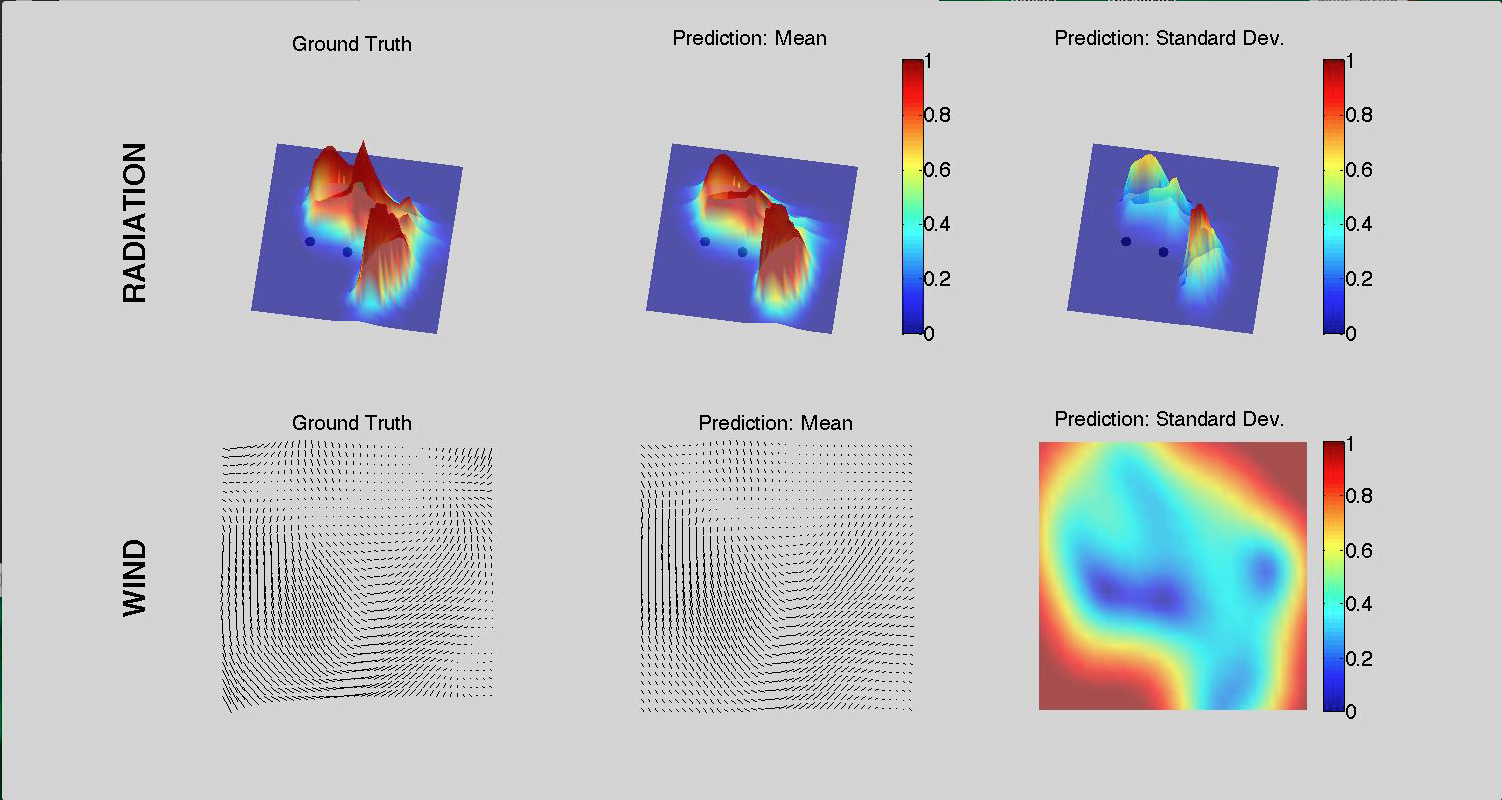
\includegraphics[width=0.45\textwidth]{figures/radiation_ss_calm.png}\\
%    (a) Slowly varying wind conditions\\ \ \\
%    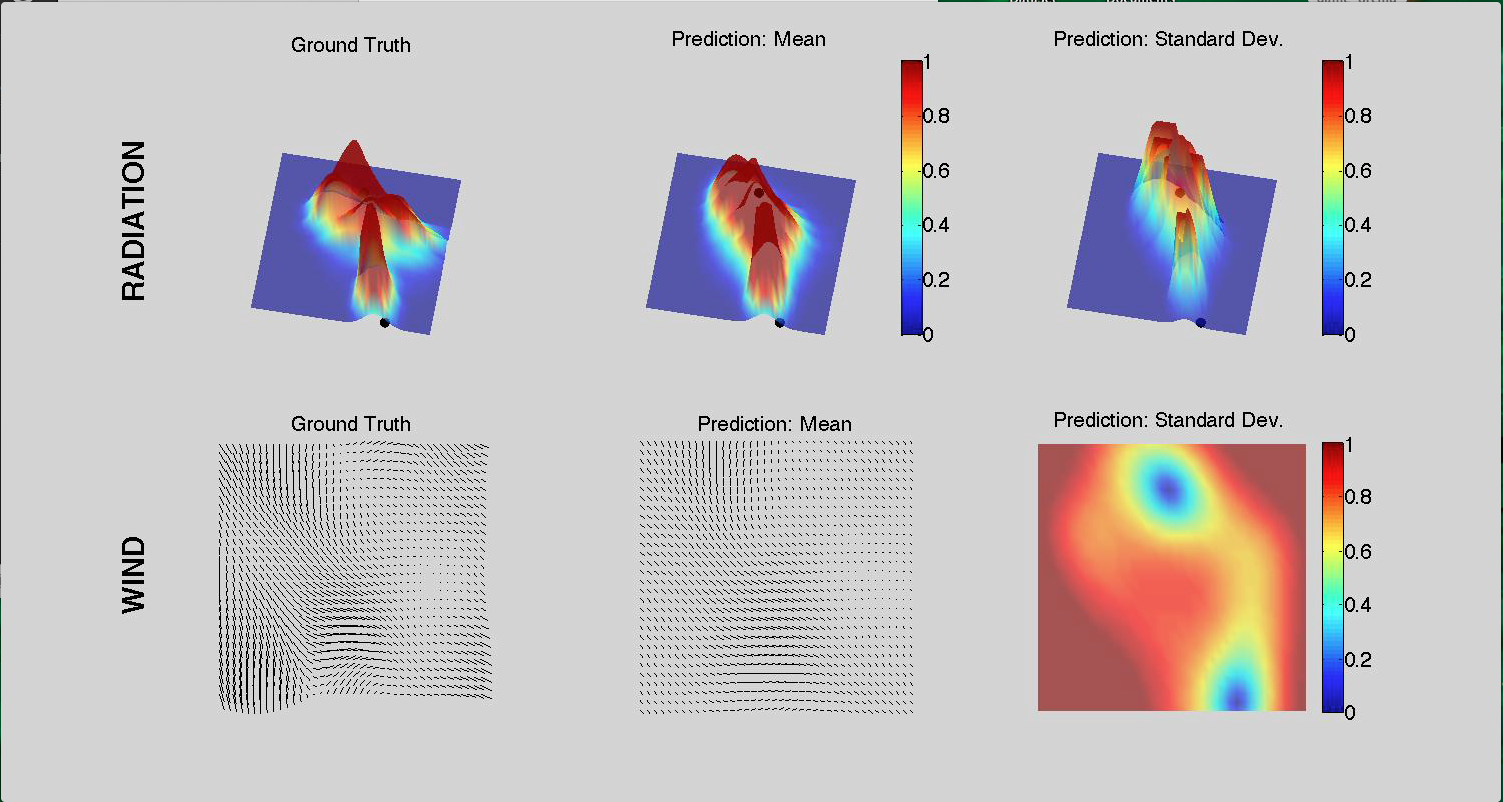
\includegraphics[width=0.45\textwidth]{figures/radiation_ss_gust.png}\\
%    (b) Gusty wind conditions 
%\caption{\label{radiation_screen_shots} Radiation and wind simulation ground truth and EKF estimates obtained using measurements from monitor agents (black dots).  Left most panes are ground truth radiation and wind conditions, the middle panes are corresponding estimates and right most panes are state uncertainties:  (a) Invariant and (b) gusty wind conditions.}
%\end{center}
%\end{figure}





\section{Real-world evaluation}
[Note: currently not sure whether to include the non-agent runs. Problematic because: a) unequal number of responders, b) HQ staffed by students in non-agent condition; researchers in agent-condition, c) not enough cases for a quantitative comparison anyways?.]
(\textbf{Joel: the population type does not matter so much for AAMAS as tar as I've seen. So go ahead with the analysis of the no-agent condition.})
We ran four sessions of AtomicOrchid with participants recruited from the local university to evaluate mixed-initiative coordination in a disaster response scenario. The following sections describe the participants, procedure, session configuration and methods used to collect and analyse quantitative and qualitative data.

\subsection{Participants}
A total of 29 participants (XX of them were female) were recruited through posters and emails, and reimbursed with 15 pounds for 1.5-2 hours of study. The majority were students of the local university. [Say something about their map reading skills?]

\subsection{Procedure}
The procedure consisted of 30 minutes of game play, and about 1 hour of pre-game briefing, consent forms and a short training session, and post-game group discussion and questionnaire. 

%Upon arrival in the HQ (set up in a meeting room at the local university), participants were briefed and asked to consent to participate. They were presented with a demographic questionnaire to record gender, occupation, experience of using smartphones and level of map navigation skills.

At the end of the briefing in which mission objectives and rules were outlined, responder roles were randomly assigned to all participants (fire-fighter, medic, transporter, soldier). HQ in the agent condition was staffed by a different member of the research team in each session in order to mimick an experienced HQ whilst avoiding the same person running HQ every time. 

Field responders were provided with a smartphone; HQ coordinators with a laptop. The team was given 5 minutes to discuss a common game strategy. (\textbf{Joel: where did the agent run ?})

Field responders were then accompanied to the starting point within the designated game area, about 1 minute walk from headquarters. Once field responders were ready to start, HQ sent a `game start' message. After 30 minutes of game play the field responders returned to the HQ for the post-game session, which consisted of a questionnaire aimed at collecting participants' feedback on (1) first impressions of the game; (2) usability of the system, and; (3) coordination issues in the game. A group interview was then conducted, before participants were debriefed and dismissed.

\subsection{Game sessions}
We ran two sessions without the planner agent, and two sessions with the planner agent to be able to compare team performance in the two conditions. We also ran a pilot study for each condition. The pilot study showed that this was a challenging, yet not too overwhelming number of targets to collect in a 30 min game session. There were four targets for each of the four target types.
The target locations, pattern of cloud movement and expansion were kept constant for all game sessions. 

The role allocation of the 8 field responders per session is depicted in table XX. One of the non-agent sessions only had 5 field responders due to drop outs. 

The terrain of the game area includes grassland, a lake, buildings, roads, and footpaths and lawns (see figure XX). There are two drop off zones and 16 targets.

\subsection{Methods}
We took a mixed methods approach to data collection and analysis. In addition to quantitative questionnaires, a semi-structured group interview was conducted that aimed at eliciting important decision points, strategies and the overall decision-making process. Furthermore, researchers with camcorders recorded the game play. One researcher recorded action in the HQ, and four other researchers each shadowed a field responder team with a camcorder.

We developed a log file replay tool to help with data analysis of time stamped system logs that contain a complete record of the game play, including responders' GPS location, their health status and radioactive exposure, messages, cloud location, locations of target objects and task status.

Video recordings of field action were catalogued to identify sequences (episodes) of interest (cf. Heath et al., 2010). Key decision points in teaming and task allocation served to index the episodes. Interesting distinct units of interaction were transcribed and triangulated with log files of relevant game activity for deeper analysis. Due to space constraints we can only  present one fragment in this paper to illustrate how human-agent collaboration typically unfolded (TODO).

How are remote messages used as a coordination resource? We use speech-act theory (Searle, 1975) to classify messages sent between and among responders and HQ. We focus on the most relevant types of acts in this paper (which are also the most frequently used in AtomicOrchid):

\begin{itemize}
\item Assertives: \textit{speech acts that commit a speaker to the truth of the expressed proposition}; these were a common category as they include messages that contain situational information.
\item Directives: \textit{speech acts that are meant to cause the hearer to take a particular action}, e.g. requests, commands and advice, including task and team allocation messages. 
\end{itemize}

\subsection{Results}

\paragraph{Structure}
\begin{itemize}
\item  \textit{Overall performance}. Draw on metrics below: tasks completed, number and categorisation of messages (only directives and assertives).


task finished in 1 pp in agent-enabled session [session a 8] 
task finished in 1.43 pp in agent-enabled session [session b 12, session c 11]

number of team reformation are 6 in the non-agent session 
average number of team reformation are 6.5 in agent-enabled session [session b 4 , session c 9]

The avg health in agent condition is 80.75 (session b 79.75, session c 81.75)
The avg health in non-agent condition is 39.695

\item \textit{Agent performance}. Metrics from below: Number of instructions sent, robustness etc. 
Replan happened 32 times across 2 agent-enabled sessions [14,18]. Triggered by rejection 8 times, triggered by drop off 24 times [1 unsuccessful drop off, 23 successful drop off]


[2 diagrams are ready agent teaming instruction, HQ directives classification, observed 4 violations of agent planning]. 

\item \textit{Task allocation}: How task allocation unfolded in the agent vs. non-agent condition. (Message handling (from JSCWS paper) vs. task handling diagram...) This is where we'd show a fragment to illustrate? -> Shows overall performance increase in performance
[begin looking for fragments now]


\item \textit{Rejecting tasks}: When and why did it happen? (-> pick this up in the discussion re. Gopal's/Feng's point on adjustable planning?). 
11 rejections happened in two sessions. All rejections happened when the planning agent tried to split existing teams, and instructing them to team up with distant players. In most cases (9 out of 11), the rejection will lead to an adapted plan which consistent with their current teaming. In the other 2 cases, players consecutively reject plan twice in order to get the satisfactory plan. 
 

Players are more likely to reject plan if their proposed teammates are far away from them.
For accepted instructions, the average distance between related players are 12 meters.
For rejected instructions, the average distance between related players are 86 meters.

\item \textit{The role of HQ}: monitoring, supporting and dealing with contingencies. Some example messages. Draw on HQ metrics. (-> Shows division of labour and the benefits of human-agent collaboration).
HQ have to click "view" button to reveal agent plan. We observed 57 clicks in the 2 agent-enabled sessions. 

\end{itemize} 
 
Joel and Wenchao
\begin{enumerate}
\item Explain setup of experiment - area of interest + setup of tasks
\item Explain evaluation = quantitative and qualitative.
\end{enumerate}
\paragraph{Metrics}
\begin{itemize}
\item{Comparisons between with/without agent versions for the below:}
\item{Performance of FR: number of tasks completed, time on task?, number of messages sent, number of teams formed and disbanded, time on team, acknowledgements of tasks}
\item{Messages: classification}
\item{Health}
\item{Distance travelled}
\item{HQ: number of agent monitoring actions (clicks), number of 'supporting'/related messages (e.g., enforcement, contradictions/overriding)}
\item{Agent performance: number of instructions, number of replanning steps, replanning robustness (diversion of task allocation compared to previous step)}
\item{Following instructions ('obedience'): number of instructions followed vs. not followed (incl. number of HQ interventions/overriding agent allocation), instruction handling diagram}
\item
\end{itemize}

\vspace{-2mm}
\section{Conclusions}\label{sec:conclusions}
\noindent In this paper we developed a novel approach for integrating and evaluating agent-based coordination algorithms that allocate teams of emergency responders in dynamic and uncertain environments.  In particular, developed a planning agent (using an MMDP approach), and conducted field-trials of a task planning agent using a mixed-reality game  called AtomicOrchid in order to focus on the issues that arise in human-agent collaboration in team coordination.

Results from our study indicate  the planning agent instructed players to carry out successful plans (outperforming a no-agent setting in terms of tasks completed and responders unharmed). The agent's ability to re-plan  as per responders' preferences and constraints was particularly effective. In particular, based on our analysis, we propose the following design guidelines for human-agent collaboration in Human-Agent Collectives:\\

\noindent \textbf{Adaptivity}: our experiences suggest that planning algorithms should be designed to take in human input, and more importantly, be \emph{responsive} to the needs of the users. As we saw in AtomicOrchid, players repeatedly requested new tasks and this would not have been possible unless our algorithm  was computationally efficient but could dynamically assimilate updates, requests, and constraints. We believe this makes the algorithm more acceptable to the users. However, this adaptivity does cost the system in terms of efficiency as the rejection of tasks may lead the problem to be so constrained that the algorithm cannot return any solutions. To alleviate such issues, we believe human mediation may be important in nudging the players to justify their rejection of tasks or to nudge them not to do so too frequently. \\

\noindent \textbf{Interaction Simplicity}: our agent was designed to issue simple commands (Do X with Y) and respond to simple requests (OK or Reject Task). Such simple messages were shown to be far more effective at guiding players to do the right task than the unstructured human communication in the non-agent assisted case that was fraught with inconsistencies and inaccuracies. In fact, we would suggest that agents should be designed with minimal options to simplify the reasoning users have to do to interact with the agent, particularly when they are under pressure to act. However, interaction simplicity in this context to us also means providing human responders with interactive abilities to do what they are good at: dealing with unforeseen contingencies. Hence, it is important to provide unconstrained communication means such as chat, walkie talkies or mobile phones in addition to the `simple' instructions that the agent provides. In effect, we are designing an interactional setting in which the agent is dealing with the routine and predictable aspects of the setting (repetitive tasks assignments), and the human coordinators in the HQ are freed up to deal with contingencies and the less predictable complexities as and when they arise.\\

\noindent \textbf{Flexbile autonomy}: the HQ dashboard proved to be a key tool for the HQ coordinator $H$ to \emph{check} and \emph{correct for} the allocations of $PA$, taking into account the real-world constraints that the players on the ground faced. In particular, letting the human oversee the agent (i.e., ``on-the-loop") at times and actively instructing  the players (and bypassing the agent) at other times (i.e., ``in-the-loop") as and when needed, was seen to be particularly effective. This was achieved by $H$ \emph{without the agent} defining when such transfers of control should happen (as in \cite{scerri:etal:2005}) and, therefore, left the coordinator the option of taking control when she judged it was needed. However, while this allows humans to \emph{choose} what to do, it is not clear whether they would have been better off going with the agent's plan. Hence, we suggest that such deployed autonomous systems should be built for flexible autonomy. Specifically, interfaces should be designed to pass control \emph{seamlessly} between humans and agents and the implications of human-based ``corrective'' actions  should be made explicit to the humans to ensure they know when to take control, and when to let the agent decide.

Much remains to be done to further validate agent-based planning in real-world disaster response given that field trials of AtomicOrchid are limited to using volunteers and in settings that only approximate the typical environments faced by emergency responders. Hence, in future work, we aim to deploy our planning agent to support expert emergency responders from RescueGlobal during their annual multi-national disaster response training exercise  (Angel Thunder\footnote{http://www.dm.af.mil/library/angelthunder2013.asp.}). By so doing, we will develop new requirements for agent-based technologies for settings where users are highly trained and the actions taken by the agent can have major impact on the performance of the team (e.g., leading to loss of lives or waste of real resources).



\clearpage
\bibliographystyle{aaai}
\fontsize{9.5pt}{10.5pt}
{

\bibliography{citations}
}


\end{document}
